\documentclass{article}
\usepackage[margin=1in]{geometry}
\usepackage{enumerate}
\usepackage{graphicx}

\graphicspath{{./images/}}


\title{Assignment 4}
\author{Marato Gebremichael}
\date{Due 5/11/2020}

\begin{document}
   \maketitle
   
\section*{Problem 1}   

\begin{enumerate}[(a)]

\item Actors:

   \begin{itemize}
      \item Companies - will use to post jobs with requirements and expected salary 
      \item Applicants (candidates) - will post their resume and generate their profiles
      \item Moderator staff - will review and approve job posts and applicants profiles
      \item Site owners - has a monetary interest in a successful job board
      \item Developers - builds the job boards
      \item Job board (system) - matches suitable candidates to jobs
   \end{itemize}

\item Use cases:
  
 \begin{table}[htbp]
	\centering
	\begin{tabular}{lllll}
		\textbf{Actors}  & \textbf{Use Case Description} &  &  &  \\
		
		Companies, Moderator staff             & Posts job posting                 &  &  &  \\
		Companies, Moderator staff             & Updates job posting               &  &  &  \\
		Companies, Moderator staff             & Closes job posting                &  &  &  \\
		Applicants, Moderator staff, Companies & Views job posting                 &  &  &  \\
		Applicants                             & Applies to a job                  &  &  &  \\
		Applicants                             & Posts resume to job board         &  &  &  \\
		Applicants, Moderator staff            & Creates applicant's profile       &  &  &  \\
		Applicants, Moderator staff            & Updates applicant's profile       &  &  &  \\
		Job board                              & Matches applicants to job post    &  &  &  \\
		Moderator staff                        & Approves job postings             &  &  &  \\
		Moderator staff                        & Approves applicants profiles      &  &  &  \\
		Moderator staff                        & Deletes (bans) employers          &  &  &  \\
		Moderator staff                        & Deletes (bans) applicants profile &  &  &  \\
		Developers                             & Builds job boards                 &  &  &  \\
		Site owners                            & Sets terms of service             &  &  & 
		
	\end{tabular}
\end{table}

\end{enumerate} 

\newpage
\section*{Problem 2}   

\begin{figure}[h]
	\centering
	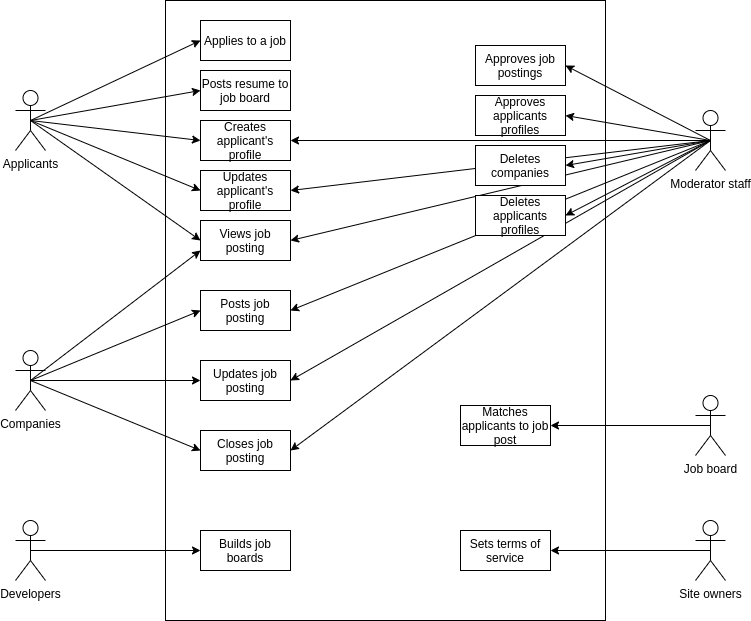
\includegraphics[scale=0.65]{Assignment_4.2_UseCaseDiagram.png}
	\caption{Use cases from Problem 1(b)}
	\label{Use Cases}
\end{figure}

\newpage

\section*{Problem 3} 

\begin{figure}[h]
	\centering
	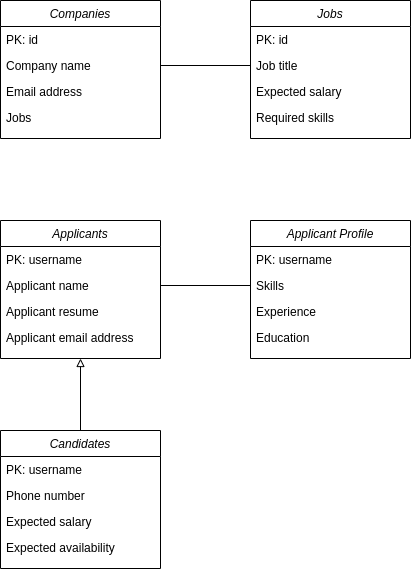
\includegraphics[scale=0.65]{Assignment _4.3_DataClasses.png}
	\caption{Expected Data Classes}
	\label{Data Classes}
\end{figure}

\begin{itemize}
	\item Companies is a "has a" relationship with Jobs data class
	\item Applicants also has a "has a" relationship with Applicant Profile data class
	\item Candidates is a subclass of Applicants data class, thus is "is a" relationship
\end{itemize}

\end{document}